\chapter{The provisioning of the infrastructure}

\section*{Introduction}
\noindent
The first sprint of this project focused on provisioning the necessary cloud resources and setting the connections between them. In this chapter, we will present how we customized the architecture to our needs and the challenges we faced during the process, and we will also showcase the features implemented in the IaC scripts.

\section{Sprint backlog}
\begin{longtable}[c]{
    |p{.85\textwidth}|
    p{.11\textwidth}|
    }
    \caption{Sprint 1 backlog}
    \label{tab:Sprint1_backlog}                                                                       \\
    \hline
    Define the structure and variables for the web Terraform module.                     & (2 points) \\
    \hline
    Define the structure and variables for the database Terraform module.                & (0 points) \\
    \hline
    Define the structure and variables for the storage account Terraform module.         & (1 points) \\
    \hline
    Develop Terraform code to provision a virtual network with subnets.                  & (4 points) \\
    \hline
    Implement the DNS zones for each module and set up the connections between them.     & (2 points) \\
    \hline
    Configure security groups for resources in each module.                              & (2 points) \\
    \hline
    implement the characteristics of the development environment.                        & (2 points) \\
    \hline
    Define environment-specific variables for the rest of the environments: QA and prod. & (1 points) \\
    \hline
    Deploy a simple web application to test the infrastructure.                          & (2 points) \\
    \hline
    write the necessary documentation on how to use the different workspaces.            & (2 points) \\
    \hline
    Test connectivity between the web application and the database for each environment. & (1 point)  \\
    \hline
    Configure the production environment for optimal performance.                        & (1 point)  \\
    \hline
\end{longtable}

\section{Realisation}
in this sprint we focused on provisioning the cloud infrastructure for our project. This involved defining and configuring the necessary cloud resources, setting up the connections between them.
and since the infrastructure will be used in three diffrent distinct situations, the first one being the development environment, in the dev team cant test the application , the second one is the quality assurance (QA) environment, where the application is tested thouroly by the QA team, and the last one is the production environment where the application is deployed to the public.
the code I wrote need to adapt depending on the environment while also maintaining modularity and reusability.
To promote code reusability, maintainability, and clarity, we adopted a modular approach for our Terraform configuration. This involved structuring the code into distinct modules, each encapsulating a specific aspect of the infrastructure (e.g., web app, database, storage account). This approach allows us to manage and update each module independently, and to reuse them across different environments.
Furthermore, to ensure consistency and streamline configuration changes, we grouped frequently used variables like SKU names, VNet prefixes, and subnet prefixes into a dedicated local.tf file.
This combined approach of modular structure and centralized variable management promotes efficient and well-organized Terraform configuration, fostering long-term project maintainability and scalability.

this figure \ref{fig:file_structure} shows the file structure of the terraform configuration.

\begin{figure}[H]
    \centering
    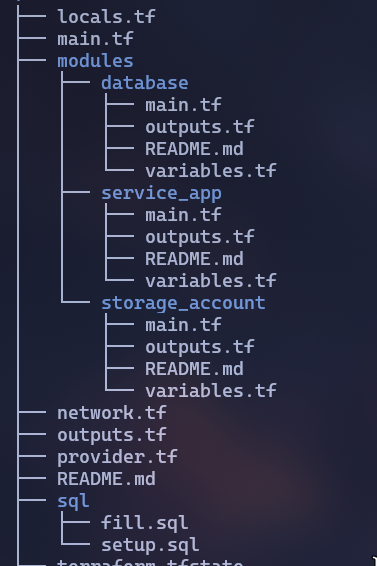
\includegraphics[width=0.3\textwidth]{file_structure.png}
    \caption{The file structure}
    \label{fig:file_structure}
\end{figure}

\subsection{the difference between the environments} 
using the terraform workspaces to manage the different environments, we can define the differences between the environments.
\begin{itemize}
    \item \textbf{dev:} the development environment:
          \begin{itemize}
              \item the resources are the most basic cost to optimize the cost.
              \item It also has a VM with a public IP inside the virtual network to access the database and the storage account.
              \item the web app and the VM can only be accessed from the CIDN given in the variables.
          \end{itemize}
    \item \textbf{QA:} the quality assurance environment:
          \begin{itemize}
              \item the resources are a bit more expensive to better simulate the production environment.
              \item It also has a VM with a public IP inside the virtual network to access the database and the storage account.
              \item it is open to the public.
          \end{itemize}
    \item \textbf{prod:} the production environment.
          \begin{itemize}
              \item the resources are the most expensive to ensure the best performance.
              \item it is open to the public.
          \end{itemize}
\end{itemize}


\subsection{The modified architecture:}
a slight modification made to the original architecture consists of the removal of the application gateway due to its high price so the user will just have to access the web app directly which is acceptable since we only have one web app.
\\ the changes in the architecture are shown in figure \ref{fig:new_arch}.

\begin{figure}[H]
    \centering
    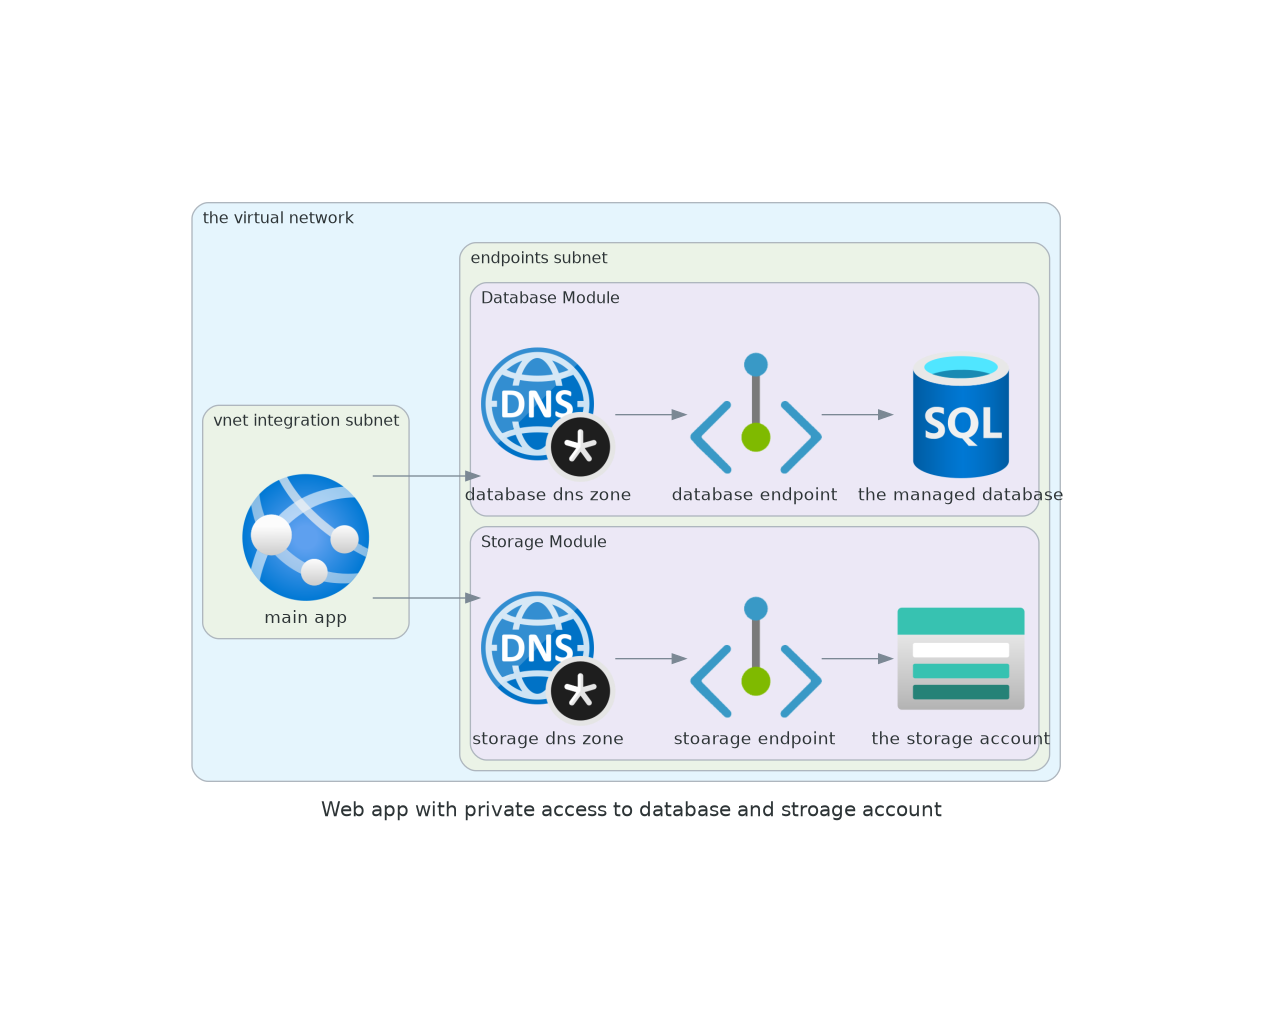
\includegraphics[width=0.8\textwidth]{web_app_with_private_access_to_database_and_stroage_account.png}
    \caption{The new architecture}
    \label{fig:new_arch}
\end{figure}


\section{Challenges}
\subsection*{ \textbullet\ The problem}
The main challenge we faced during Sprint 1 was configuring the DNS zones to enable communication between the web application and the database. Despite successfully provisioning the necessary cloud resources, the web application encountered issues resolving the hostname of the database. This meant the application couldn't locate the database to retrieve or store data, hindering core functionality. Troubleshooting involved verifying several aspects:

\begin{figure}[H]
    \centering
    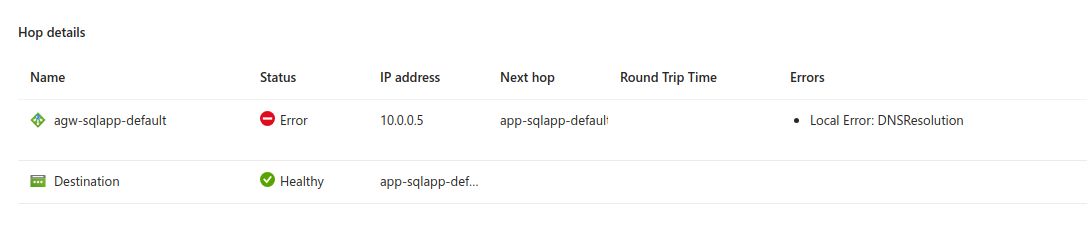
\includegraphics[width=0.8\textwidth]{connnectivity_problem.png}
    \caption{connnectivity problem}
    \label{fig:connection_problem}
\end{figure}

\begin{itemize}
    \item \textbf{DNS record configuration:} We double-checked the DNS record types (likely A record) and their values (database hostname and IP address) within the configured DNS zone. Any typos or incorrect mappings could have caused resolution issues.
    \item \textbf{Network security group (NSG) rules:} We had to verify the NSG rules to ensure the web application could communicate with the database.
    \item \textbf{verify connections:} We had to verify that the database was accessible from the web application. and that the web could access the DNS server.
\end{itemize}
By systematically examining these potential causes, we were able to identify that the web app did not have access to the DNS server provided by Azure. This experience highlights the importance of careful configuration and understanding of how DNS plays a crucial role in enabling communication between different components within a cloud infrastructure.
\subsection*{ \textbullet\ The solution}
To address the DNS resolution issue between the web application and the database, we capitalized on a core Azure concept: \textbf{the Wire Server}. This managed DNS server, automatically created within each virtual network, plays a critical role in resolving internal DNS queries using private DNS zones. Although offered as a free service, the Wire Server isn't automatically configured as the default DNS server for the virtual network.

\begin{figure}[H]
    \centering
    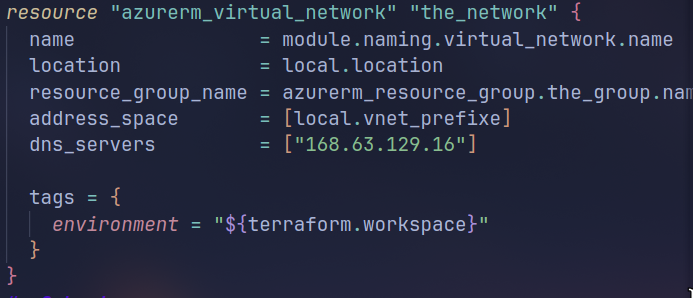
\includegraphics[width=0.7\textwidth]{DNS_server.png}
    \caption{The DNS configuration}
    \label{fig:dns_configuration}
\end{figure}

Our solution involved leveraging Terraform to explicitly set the Wire Server's static IP address (168.63.129.16) as the default DNS server within our virtual network configuration. By making this configuration change, we ensured that the web application could effectively utilize the Wire Server to resolve the database hostname and establish the necessary communication channel. This approach eliminated the initial DNS resolution obstacle and facilitated seamless communication between the application and the database.

\section{Testing the connections}
\subsection*{ \textbullet\ The user to the application}
To test the connectivity between the web application and the user, I deployed a simple web application that displays a welcome message. We then accessed the web application using a web browser to verify that the application was accessible from the designated CIDR range in the development environment.
\subsection*{ \textbullet\ The application to the database}
To test the connectivity between the web application and the database, I used the Azure Portal to verify that the web application could successfully communicate with the database. This involved checking the database connection status and ensuring that the web application could read and write data to the database.
\subsection*{ \textbullet\ Integration testing}
To ensure that the web application and database could communicate effectively, I performed integration testing by simulating user interactions with the application. This involved submitting data through the web application and verifying that the data was correctly stored and retrieved from the database. By testing the end-to-end functionality of the application, I confirmed that the web application and database were successfully connected and operational.
\begin{figure}[H]
    \centering
    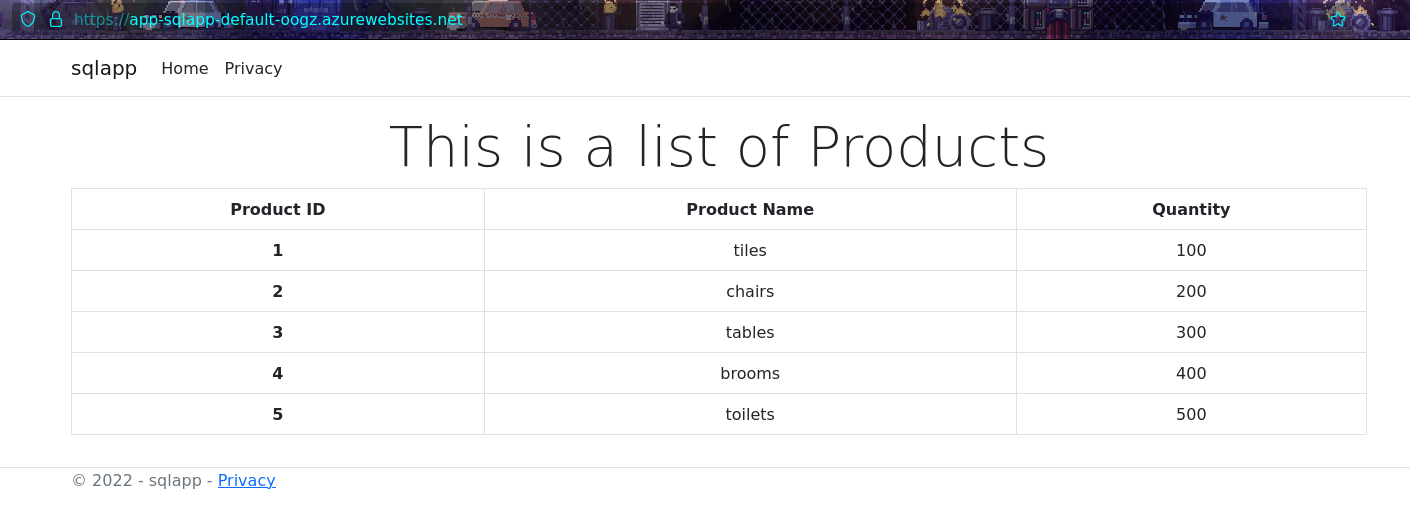
\includegraphics[width=0.8\textwidth]{integration_testing.png}
    \caption{the simple web app that was used to test the infrastructure.}
    \label{fig:testing}
\end{figure}

\section*{Conclusion}
This chapter detailed the successful completion of Sprint 1, focusing on provisioning the cloud infrastructure for our project. We presented a modified architecture that removed the application gateway due to cost considerations. The new architecture leverages Terraform modules for efficient code organization and utilizes workspaces to manage different environments (dev, QA, prod) with appropriate resource configurations.
\par
We encountered a challenge during this sprint related to DNS configuration, where the web application struggled to resolve the database hostname. This issue was resolved by leveraging the Azure Wire Server as the default DNS server within the virtual network configuration.
\par
By successfully provisioning the infrastructure and addressing the DNS resolution challenge, Sprint 1 laid the foundation for future sprints to focus on building and deploying the web application and its functionalities within the cloud environment as will be detailed in the next chapter.
